\documentclass[a4paper]{article}
\usepackage{wrapfig}
\usepackage[eng,exjobb]{KTHEEtitlepage}
\usepackage[cp1252]{inputenc}
\usepackage[english]{babel}
\usepackage{fancyhdr}
\usepackage{graphicx}
\usepackage[table,xcdraw]{xcolor}
\usepackage{float}
\usepackage{adjustbox}
\usepackage{ amssymb }
\usepackage{hyperref}

\usepackage{biblatex}
\addbibresource{reference.bib}
\pagestyle{fancy}
\fancyhf{}
\rhead{}
\lhead{Sound based research on clock-shifting the Manx shearwater}
\rfoot{Page \thepage}


\begin{document}

                \ititle{Research Project}
              % \isubtitle{Julian Main, Lucas Van Berkel, Yorick De Boer, Amor Frans} % Optional
                \idate{Januari 2016}
                \irefnr{}
                \iauthor{\large{Sound based research on clock-shifting the Manx shearwater}}
                
                \makeititle

\newpage

%%%%%%%%%%%%%%%%%%
\tableofcontents
\newpage
%%%%%%%%%%%%%%%%%%
\begin{abstract}
    The purpose of this project is to support a research on biological clock and sun based navigation of the Manx shearwater. To influence the birds navigation an attempt was made to shift the birds clock using light manipulation. In addition to the main GPS based research, this research focuses on the bird while still inside its burrow. Using audio recordings from inside the birds burrow, we try to find patterns in the birds behaviour using machine learning. The goal of this is, to see if the birds pattern shifts when the time is shifted. Although the results of this research on whether the clock-shift worked are inconclusive, there are signs that the clock-shift might have worked.

\end{abstract}
%%%%%%%%%%%%%%%%%%
\addcontentsline{toc}{section}{Introduction}
\section*{Introduction}
The subject of this project is to determine if a clock-shift has occurred on Manx shearwaters in an experiment held last summer in 2015. The experiment manipulated 8 Manx shearwaters into shifting its biological clock. The research conducted here is commissioned by the Institute for Biodiversity and Ecosystem Dynamics. The institute is represented by Oliver Padget, a PhD student of the university of Oxford, helped by the dutch associate dr. ir. Emiel van Loon, Assistant Professor on statistical ecology. The same project was conducted last year by a different group, but the results were unable to give a satisfying answer to the main question of the institute.\\\\
 The Manx Shearwater is a black and white seabird which nests in burrows. This bird nests on islands in the northeast Atlantic. In July, after the breeding period, the birds will migrate to the South-Atlantic and will return again in March the following year. During the breeding period one of the parents will stay with the eggs during a period of 7 to 12 days, while the other parent will search for food. After these 7-12 days the parents will swap roles.\\\\ 
The main goal of the experiment held in 2015 was to prove that the Manx shearwater uses the sun while migrating. In order to test if the Manx shearwater uses the sun as a compass while migrating over sea, the tested birds were manipulated, changing their endogenous clock four hours forwards or backwards. For the clock-shift the burrows were closed for nine days and artificial light was placed in the burrow. For the first six days the time when the light was on, would match the time when the sun was up. After the six days the clock-shift was executed and the time when the light was on would differ four hours from the time when the sun was up. The clock-shift is a good test because if the Manx shearwater uses the sun as a compass then the bird needs a precise endogenous clock to navigate.After the clock-shifting has occurred, the birds were released some distance from their burrows on sea with GPS-tracking, to see what kind of path the birds took. To prove the clock-shifting has successfully occurred, some birds were manipulated the same way, but with a microphone in the burrow. If the Manx shearwater was clock-shifted, the researchers presumed its sound-pattern would change the same way. Therefore the main question of this research was to prove whether it was possible to show that the bird was successfully manipulated through the audio recordings.\\\\
Last years group calculated the most dominant frequency, the activity over a period of time using the amplitude as threshold, the average amplitude over a period of time and the band power. Five minutes was the chosen step time, so every interval provided enough information to calculate each feature. The result of the previous research concluded that the results were not reliable enough to determine whether the birds were clock-shifted or not.


%%%%%%%%%%%%%%%%%%
\addcontentsline{toc}{subsection}{Problem}
\section*{Problem description}
As stated before, the main subject was to determine if the clock-shift had worked. Recordings were made in 8 burrows. In each of these burrows a clock-shift was performed. Two types of clock-shifts were used: a 4 hour forward shift(shift-fast), and a 4 hour shift backward shift(shift-slow). Audio recordings of 8 different birds were provided. Each microphone of each bird produced 9 audio files. One audio file for every day of the experiment. For the first six days the time when the light was on, would match the time when the sun was up. In the last three days the clock would be shifted backwards or forward. The recordings were not complete for all burrows.
\begin{table}[H]
    \centering

\begin{tabular}{l|
>{\columncolor[HTML]{FFCE93}}c 
>{\columncolor[HTML]{FFCE93}}c 
>{\columncolor[HTML]{FFCE93}}c 
>{\columncolor[HTML]{FFCE93}}c 
>{\columncolor[HTML]{FFCE93}}c 
>{\columncolor[HTML]{FFCE93}}c 
>{\columncolor[HTML]{FFCCC9}}c 
>{\columncolor[HTML]{FFCCC9}}c 
>{\columncolor[HTML]{FFCCC9}}c }
burrow & \cellcolor[HTML]{FFFFFF}{\color[HTML]{F56B00} 16/6} & \cellcolor[HTML]{FFFFFF}{\color[HTML]{F56B00} 17/6} & \cellcolor[HTML]{FFFFFF}{\color[HTML]{F56B00} 18/6} & \cellcolor[HTML]{FFFFFF}{\color[HTML]{F56B00} 19/6} & \cellcolor[HTML]{FFFFFF}{\color[HTML]{F56B00} 20/6} & \cellcolor[HTML]{FFFFFF}{\color[HTML]{F56B00} 21//6} & \cellcolor[HTML]{FFFFFF}{\color[HTML]{CB0000} 22/6} & \cellcolor[HTML]{FFFFFF}{\color[HTML]{CB0000} 23/6} & \cellcolor[HTML]{FFFFFF}{\color[HTML]{CB0000} 24/6} \\ \hline
F:B73  & $\checkmark$                                        & $\checkmark$                                        & $\checkmark$*                                       & $\checkmark$                                        & $\checkmark$                                        & $\checkmark$*                                        & {\color[HTML]{CB0000} $\checkmark$}                 & {\color[HTML]{CB0000} $\checkmark$}                 & {\color[HTML]{CB0000} $\checkmark$}                 \\
S:B151 & $\times$                                            & $\times$                                            & $\times$                                            & $\times$                                            & $\times$                                            & $\times$                                             & {\color[HTML]{CB0000} $\times$}                     & {\color[HTML]{CB0000} $\times$}                     & {\color[HTML]{CB0000} $\checkmark$}                 \\
F:B174 & $\checkmark$                                        & $\checkmark$                                        & $\checkmark$*                                       & $\checkmark$                                        & $\checkmark$                                        & \textendash                                          & {\color[HTML]{CB0000} \textendash}                  & {\color[HTML]{CB0000} $\checkmark$}                 & {\color[HTML]{CB0000} $\checkmark$}                 \\
S:B179 & $\checkmark$                                        & $\checkmark$                                        & \textendash                                         & $\checkmark^+$                                      & $\checkmark$                                        & $\checkmark$                                         & {\color[HTML]{CB0000} $\checkmark$}                 & {\color[HTML]{CB0000} $\checkmark$}                 & {\color[HTML]{CB0000} $\checkmark$}                 \\
F:DB4  & $\checkmark$                                        & $\checkmark$                                        & $\checkmark$                                        & $\checkmark$                                        & $\checkmark$                                        & Mic                                                  & {\color[HTML]{CB0000} $\checkmark$}                 & {\color[HTML]{CB0000} $\checkmark$}                 & {\color[HTML]{CB0000} $\checkmark$}                 \\
S:DB12 & $\times$                                            & $\times$                                            & $\times$                                            & $\times$                                            & $\times$                                            & $\times$                                             & {\color[HTML]{CB0000} $\times$}                     & {\color[HTML]{CB0000} $\checkmark$}                 & {\color[HTML]{CB0000} $\checkmark$}                 \\
F:DB20 & $\checkmark$                                        & \textendash                                         & $\checkmark$                                        & $\checkmark$                                        & $\checkmark$                                        & $\checkmark$\textendash                              & {\color[HTML]{CB0000} $\checkmark$}                 & {\color[HTML]{CB0000} $\checkmark$}                 & {\color[HTML]{CB0000} $\checkmark$}                 \\
S:DB30 & $\checkmark$                                        & $\checkmark$                                        & $\checkmark$                                        & $\checkmark$                                        & \textendash                                         & $\checkmark$                                         & {\color[HTML]{CB0000} $\checkmark$}                 & {\color[HTML]{CB0000} $\checkmark$}                 & {\color[HTML]{CB0000} $\times$}                    
\end{tabular}
\caption{Table of the data given by Oliver Padget,
where $\checkmark$ means full 24 hours, $\checkmark$ \textendash means between 18 and 24 hours, $\checkmark$ * means less then 18 hours. $\times$ means no recording. Mic means that microphone was not located properly. F means forward shift, S means backward shift.}
\end{table}
The presumption was that the clock-shift would not work immediately, comparable with a jet-lag for human beings. Therefore the expectation was that the clock-shift would work, but in steps of 1 hour per day. This is a note that is important for the evaluation.\\\\
The main goal of this research was to validate whether the clock-shift worked based on the audio-recordings. To validate this the following sub-questions were attempted to answer:\\
 (I)    What is the activity pattern of the Manx shearwater during 24 hours in the audio recordings? \\
 (II)   What is the difference between the unshifted days and the shifted days in the activity pattern?
 
%%%%%%%%%%%%%%%%%%
\addcontentsline{toc}{subsection}{Strategy}
\section*{Strategy}
\begin{wrapfigure}{r}{0.28\textwidth}
\vspace{-23pt}
  \begin{center}
    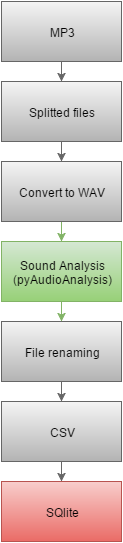
\includegraphics[width=0.13\textwidth]{diagram}
  \end{center}
  \vspace{-20pt}
  \caption{Flow chart}
\end{wrapfigure}
To determine the activity-pattern every activity in each recording was labeled. Each burrow had 24-hour of recordings for 9 days, in total approximately 216 hours of audio recording for all days. Nine burrows, so a total of 1944 hours of recordings. To solve the problem as stated before we choose to decide to follow the following strategy:\\\\
1) Preparing data \\
2) Train model to classify sounds \\
3) Abstract results from classification to usable data\\
4) Analyze results\\\\
The following chapter is a step-by-step description of how we handled these steps. 


%%%%%%%%%%%%%%%%%%
\addcontentsline{toc}{section}{Method}
\section*{Method}

\addcontentsline{toc}{subsection}{Preparing data}
\subsection*{Preparing data }
Since the provided audio files were MP3 encoded, we had to decode them to WAV format to process them. In order to make the files more workable, each recording was split into pieces of exactly one hour long. This resulted in files of approximately 1.5GB. The analyzation process of the file keeps the whole file in memory, so they could not be too big. Next the files had to be renamed so the filename represented the real date and time of the recording. 

\addcontentsline{toc}{subsection}{Train model}
\subsection*{Train model for classification }
While listening to some audio files, multiple sounds could clearly be classified. The most interesting sound was when the bird moved, this sound was named 'shuffle'. The sound that mostly identifies the Manx Shearwater is its call, but previous research showed that the bird calls mostly in anticipation of other birds\cite{brooke1978sexual}. Given that the call would not have been a good identifier of the activity pattern of the bird. Therefore we chose 'shuffling' as our identifier for the activity pattern. The constant background noise was classified as silence. We also added a class named environment noise so that we are sure that the noises from other birds will not be classified as shuffles or calls by the bird in the burrow.
Therefore we have the classifications: shuffling, calling, silence and environment noise.\\\\The trainings data was collected by searching in the audio files for shuffles, silent fragments, calls and environment noises by ear. The group of last year combined all the data of the different birds. The result of this strategy was not so good, because every burrow can differ in size and therefore the recordings can be different. Also the place of the microphone can differ for each burrow. Therefore we chose to collect trainings data for each bird separately.\\\\After collecting the training data we let an algorithm learn to recognize these sounds and make a vector over 24 hours of this classification. An open source library for the programming language Python was used (pyAudioAnalysis)\cite{giannakopoulos2015pyaudioanalysis} for this. This library  uses 34 different short-period features, in order to determine if the sound tested, matches the sound classified using the K-nearest neighbours algorithm. Some of the features the program uses are the Zero Crossing Rate, Entropy of Energy and Spectral Spread. A complete overview of every feature is provided along with the code. We chose for a stepsize of 1 second so it returns a classification of every second in the tested audio file.
\\\\A preliminary test of detecting 'shuffles' in a time frame of 241 seconds concluded that 90 percent of the 'shuffles' was detected in that time frame. \\
\begin{figure}[!ht]
  \centering
    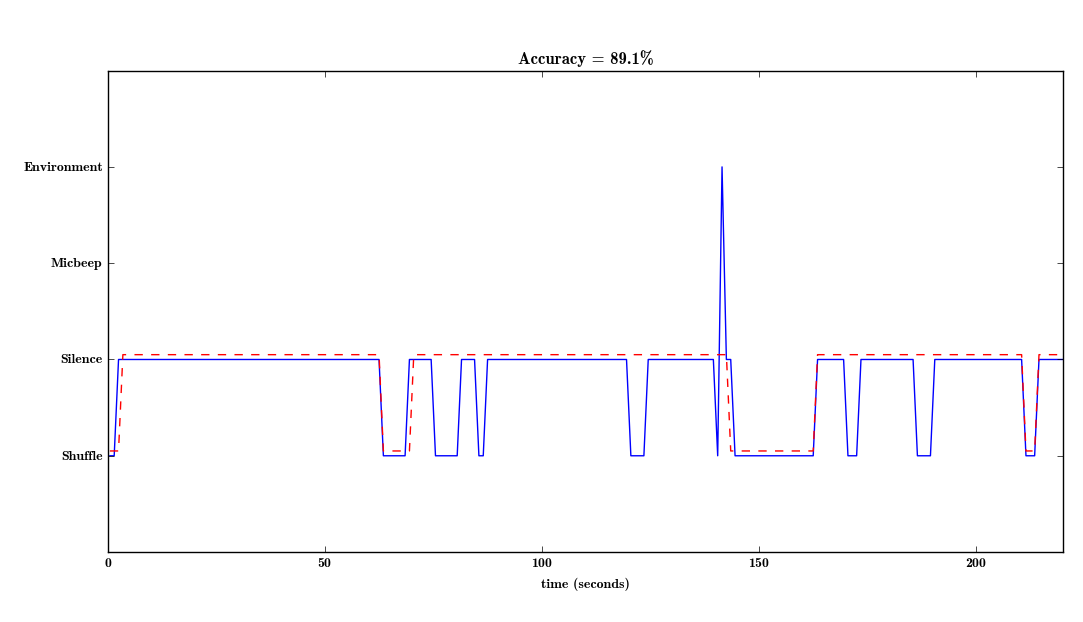
\includegraphics[width=0.9\textwidth]{accuracy_test_crop}
      \caption{Accuracy test}
\end{figure}


\addcontentsline{toc}{subsection}{Abstract to usable data}
\subsection*{Abstract to usable data}
Each audio file, approximately $9\cdot8\cdot24=1728$ in total, was run through the the audio analysis library, delivering an array of 3600 entries long. Since the microphones of two birds did not work properly for 8 days - see table 1, the results of these two birds had to be discarded. \\ \\ 
After the classification was done, every second of the audio recording then was labeled with its class and put into an array. Next every class was labeled with a timestamp and put into CSV-files (Comma-separated values files) for every bird. The CSV-files were later put into a sqllite-database (Structured Query Language Database), in order to make it easier to retrieve data from certain time points during the analysis.

\addcontentsline{toc}{subsection}{Analyze results}
\subsection*{Analyze results}
After the data was usable we first made it visible as plots. In addition to this there were two methods used to analyze the data, a interval based test and an analysis based on anomaly detection. 

\addcontentsline{toc}{subsubsection}{Confidence interval test}
\subsubsection*{Interval based test}
To validate the clockshift the shifted days must be compared with the unshifted days. We had the classifications of shuffles for each day for every hour during 24 hours. Therefore the vector of a day consist 24 variables and each variable represent the amount of shuffles in that hour. There are six vectors of the unshifted days and three vectors from the shifted day for each bird.\\\\
The idea was to separate every hour and make a confidence interval for every hour using the data from the unshifted days. And then look if the same hour in the shifted day falls in that confidence interval. After this procedure the program would shift the vector of the shifted day and repeat the procedure.\\\\ 
For example if we take hour 13, we have data how many shuffles there were in hour 13 for day 16-21(unshifted days). We put all the points of hour 13 from all the six unshifted days together . So we now have a vector of length six for hour 13, representing the amount of shuffles in hour 13 for the six days. With this vector we make a confidence interval assuming the points are distributed as a t-distribution. Say the program computes the interval 800-1200. Then the program checks if  the amount of shuffles in hour 13 on the shifted day falls into that interval. So if in hour 13 on a shifted there were 900 shuffles then the programs label this hour as a 1 if the amount of shuffles in that hour is not in the interval than the algorithm gives that hour a score of 0. \\\\
The programs repeats this procedure for every hour. At the end the program computes a percentage of the hours that falls in the confidence interval. So for example if the program returns a percentage of 50\% it means that 12 of the 24 hours fitted in the confidence interval. After this whole procedure we shifted the time-line of the shifted day by an hour and we did this four times. This is because the birds will not shift their activity immediately therefore we did check the shift of 0-4 hours. The expectation is that the birds will shift by ca. 1 hour per day so we wanted to see that the percentage of hours that falls in the confidence interval would increase by the hours of shifting. If that was the case then we could conclude that the clock-shift has worked. 

\addcontentsline{toc}{subsubsection}{Anomaly detection}
\subsubsection*{Anomaly detection}
The idea of anomaly detection is to detect anomalous points or anomalous vectors given the data. For an anomaly detection algorithm we chose to use the least-squares kernel based method.  If there are two vectors x and y then a kernel is the space of all vectors in x that will denote in the zero-vector in y. The least squares equation is an equation to compute the distance between the estimation and the real value, the idea of is that we want to minimize this distance using the algorithms and kernels. For an extensive explanation of this algorithm read this reference \cite{engel2004kernel}.\\\\
For this research the trainings data was the data of the amount of shuffles for each hour in all unshifted days, this are six vectors which each represent an unshifted day. Then a shifted day was added to the data. We did this for each shifted day. We hoped to see that this shifted vector would be flagged as anomalous before the shift because it must not fitted in the unshifted day pattern. Also we wanted to see that this shifted vector was flagged as not anomalous after the shift of 4 hours. If this was the case then we could conclude that the clock-shift worked.
%%%%%%%%%%%%%%%%%%
\addcontentsline{toc}{section}{Results}
\section*{Results}

\addcontentsline{toc}{subsection}{Classification}
\subsection*{Classification}
To make the results conceivable we made a couple of different plots. With a perfect clock shifted result the pattern of activity for 24 hours would be exactly the same for all days. When there would be a shift, the difference between the shifted days and the non shifted days would then be that the pattern also shifted. \\ \\
Unfortunately this is not the case. Although there is definitely a pattern among the activity patterns of some birds, other birds do not show a clear daily pattern. Two of the total six tested birds show a pattern which is visible when plotted.

\begin{figure}[H]
  \centering
    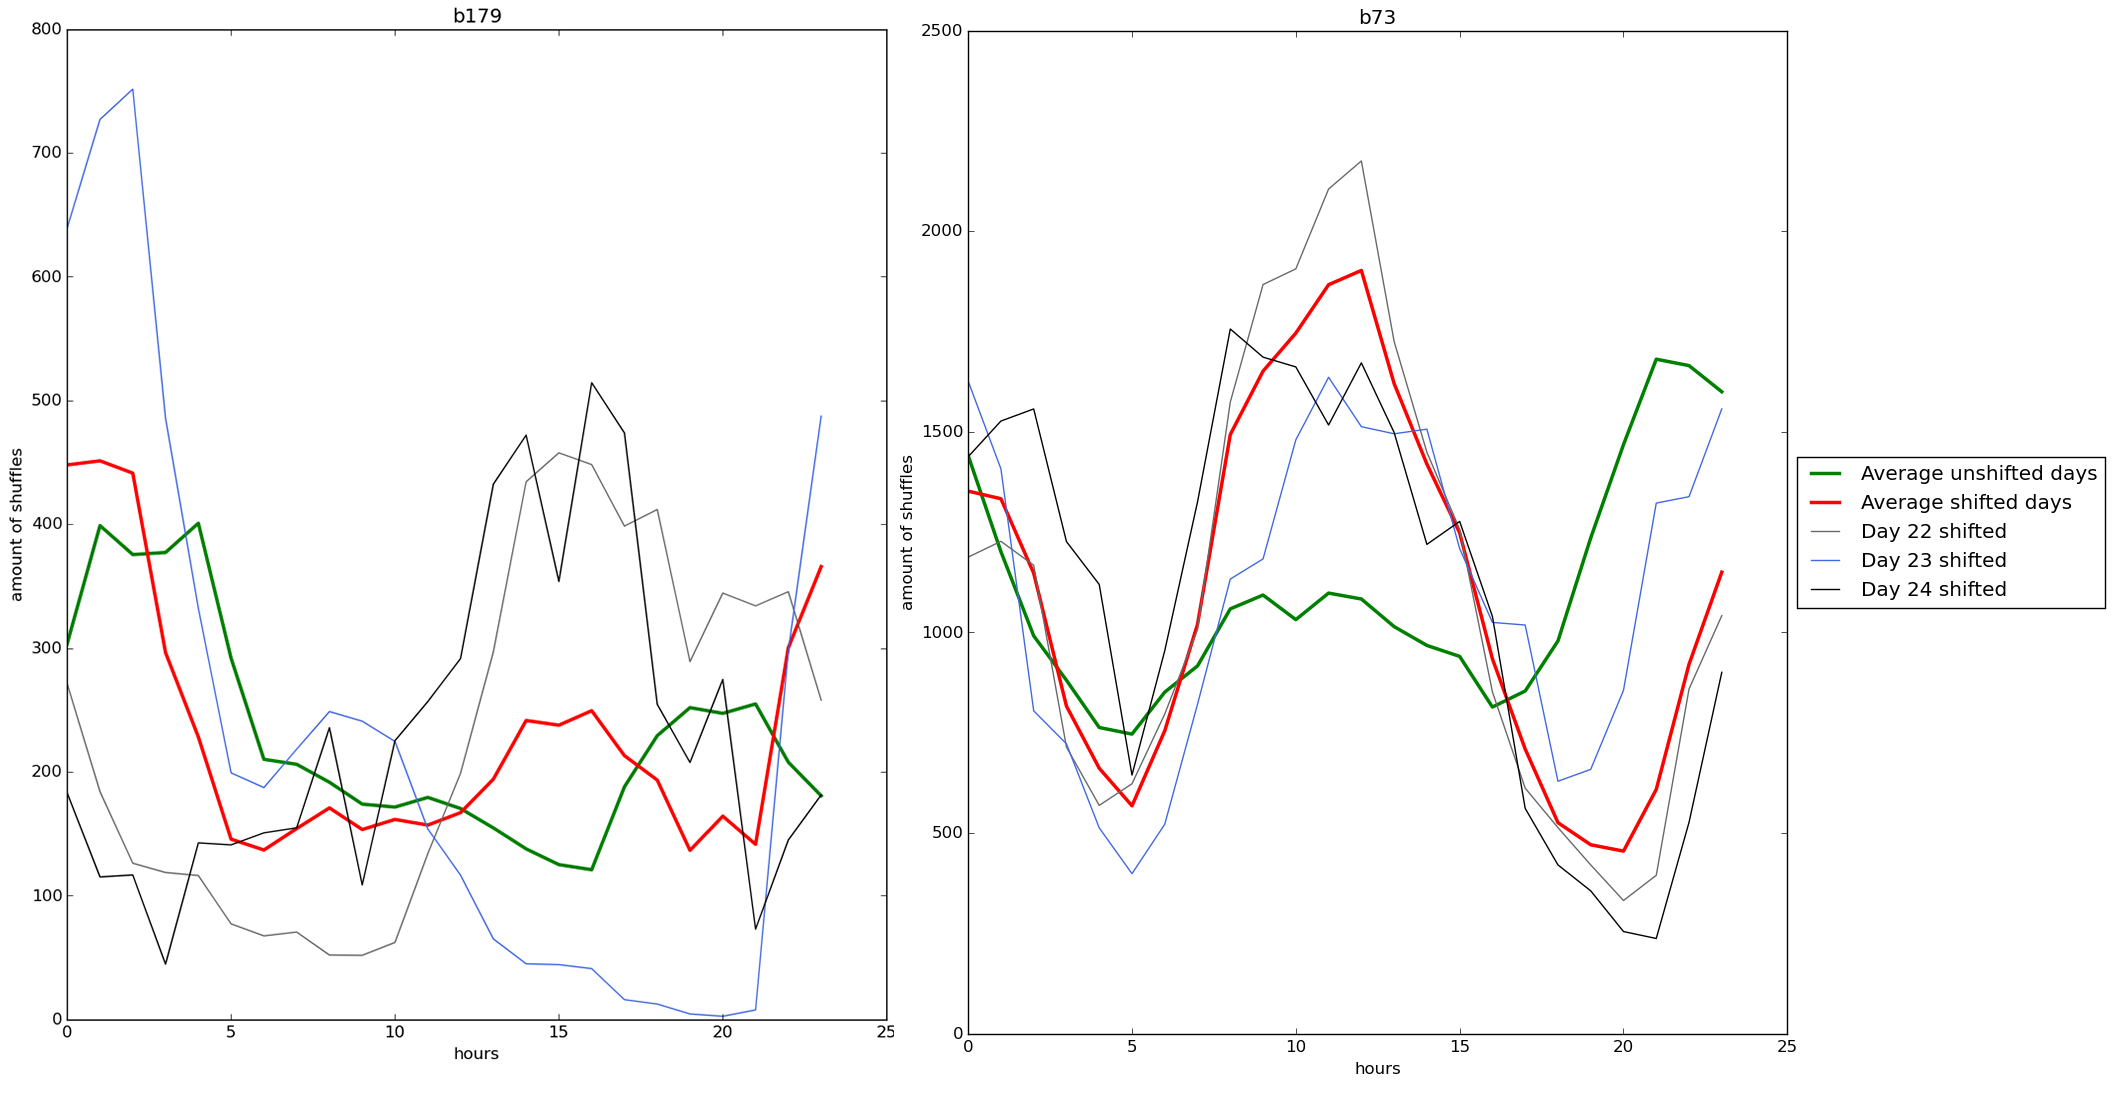
\includegraphics[width=1\textwidth]{b179_b73_merged}
      \caption{Comparison of shifted vs nonshifted days of bird b179 and b73}
\end{figure}
\\
To smooth the results we used a running mean. Also the plots were normalized so the surface under the plots is equal under each graph. This was done so the pattern among the graphs could be compared better.
\\ \\
To find out how the average of the non shifted days represents the the real value, a min-max plot was made.
\begin{figure}[H]
  \centering
    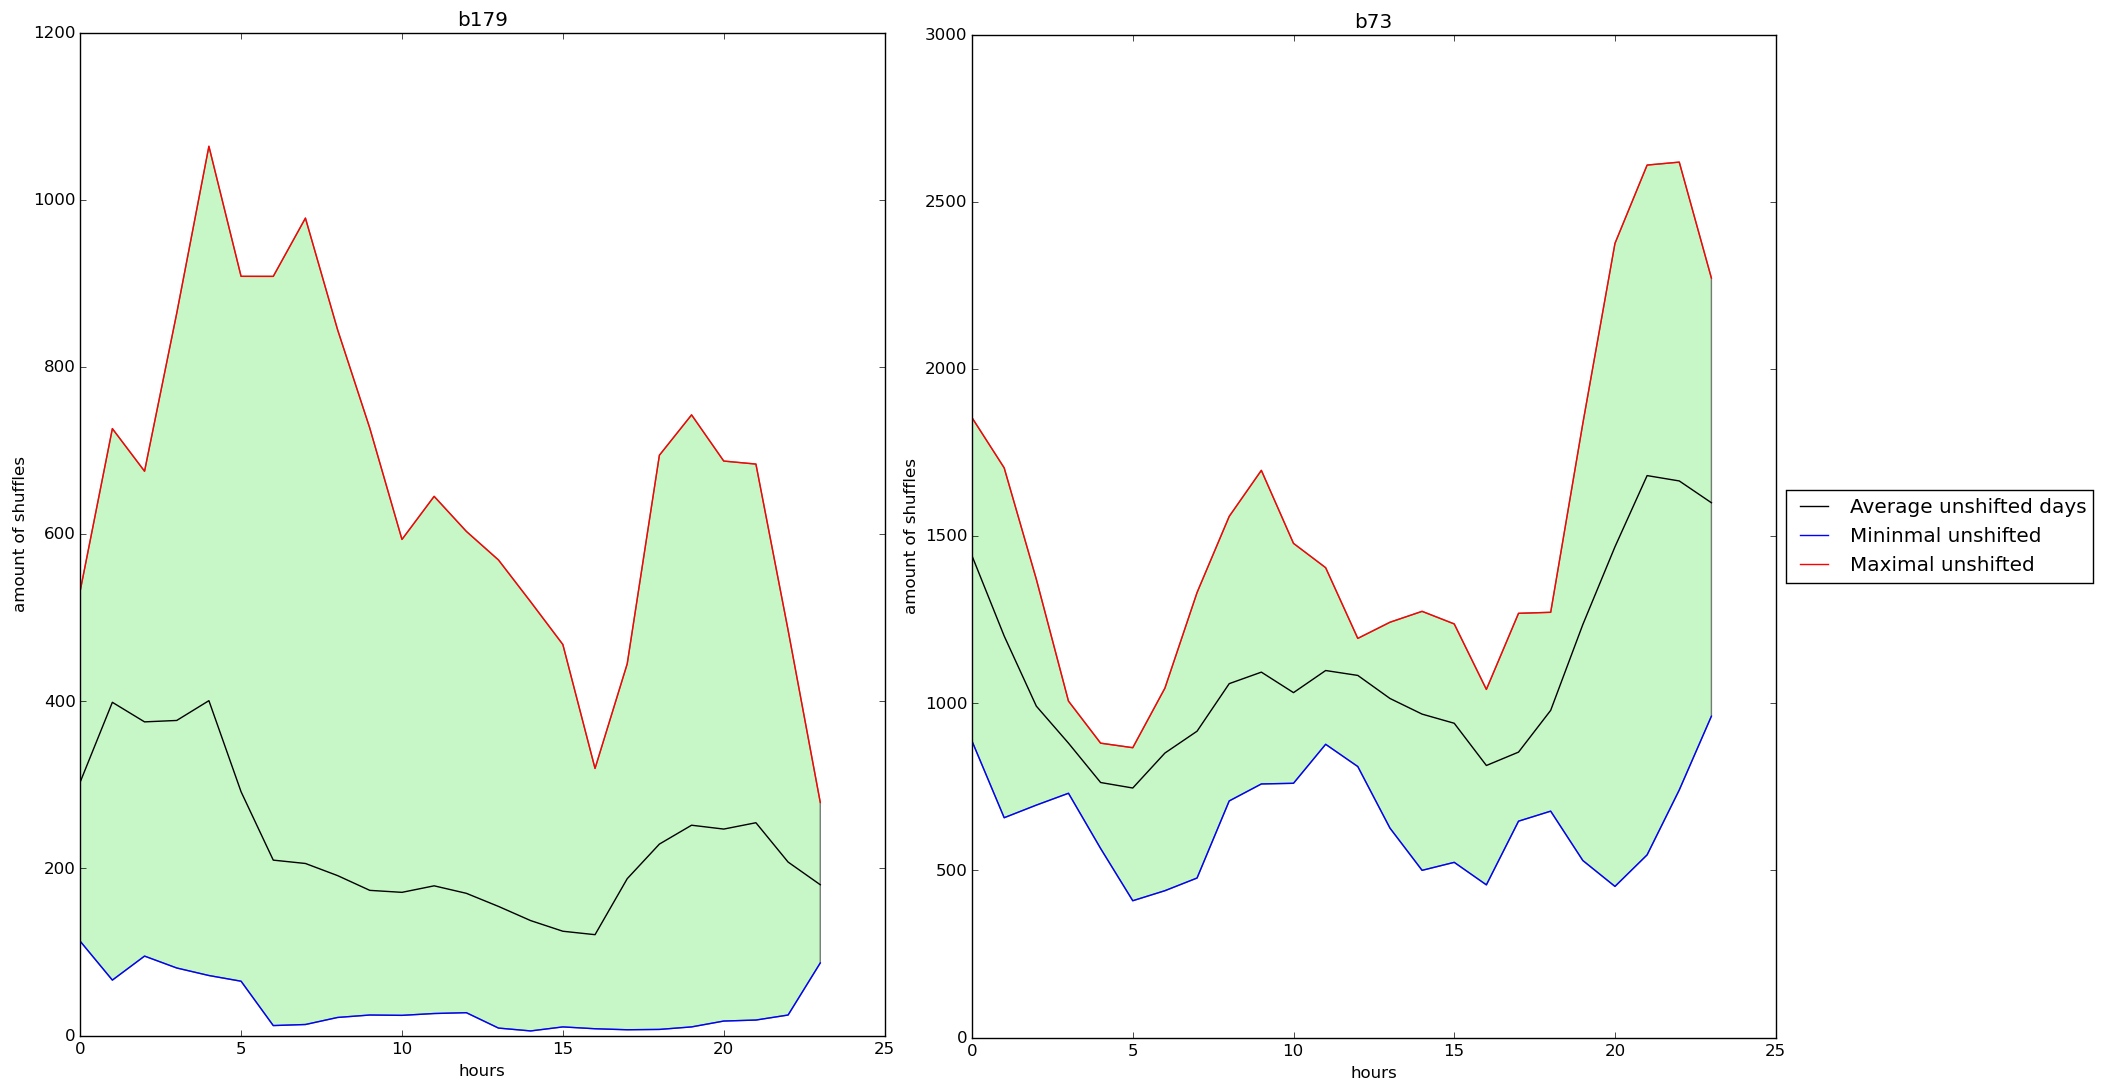
\includegraphics[width=1\textwidth]{b179_b73_merged_surface}
      \caption{Minimal and maximal values of non shifted days bird b179 and b73}
\end{figure}
It can be seen that there is a significant difference between these two birds. While the min and max values from the b73 bird are quite close the the average, the values of the b179 bird are much further apart.
\addcontentsline{toc}{subsection}{Confidence interval Test}
\subsection*{Confidence interval Test}
As stated before, we ran a test to validate whether the pattern from the shifted days and unshifted days differ significantly. This are the results of the confidence interval test:\\

\begin{table}[H]
\centering
\resizebox{\textwidth}{!}{%
\begin{tabular}{|l|l|l|l|l|l|lllll}
\hline
 & \multicolumn{5}{l|}{\textbf{Day 22}} & \multicolumn{5}{l|}{\textbf{Day 23}} \\ \hline
\textit{hours of shifting} & \textit{0} & \textit{1} & \textit{2} & \textit{3} & \textit{4} & \multicolumn{1}{l|}{\textit{0}} & \multicolumn{1}{l|}{\textit{1}} & \multicolumn{1}{l|}{\textit{2}} & \multicolumn{1}{l|}{\textit{3}} & \multicolumn{1}{l|}{\textit{4}} \\ \hline
\textbf{b73} & \cellcolor[HTML]{BBDAFF}54.167\% & \cellcolor[HTML]{FD6864}41.67\% & \cellcolor[HTML]{FD6864}45.83\% & \cellcolor[HTML]{FD6864}37.5\% & \cellcolor[HTML]{FD6864}45.83\% & \multicolumn{1}{l|}{\cellcolor[HTML]{BBDAFF}29.17\%} & \multicolumn{1}{l|}{\cellcolor[HTML]{67FD9A}41.67\%} & \multicolumn{1}{l|}{\cellcolor[HTML]{67FD9A}45.83\%} & \multicolumn{1}{l|}{\cellcolor[HTML]{67FD9A}37.5\%} & \multicolumn{1}{l|}{\cellcolor[HTML]{67FD9A}33.3\%} \\ \hline
\textbf{b174} & \cellcolor[HTML]{BBDAFF}0.0\% & \cellcolor[HTML]{FFFE65}0.0\% & \cellcolor[HTML]{67FD9A}8.33\% & \cellcolor[HTML]{67FD9A}12.5\% & \cellcolor[HTML]{67FD9A}8.33\% & \multicolumn{1}{l|}{\cellcolor[HTML]{BBDAFF}50.0\%} & \multicolumn{1}{l|}{\cellcolor[HTML]{FFFE65}50.0\%} & \multicolumn{1}{l|}{\cellcolor[HTML]{FFFE65}50.0\%} & \multicolumn{1}{l|}{\cellcolor[HTML]{FD6864}45.83\%} & \multicolumn{1}{l|}{\cellcolor[HTML]{FD6864}45.83\%} \\ \hline
\textbf{b179} & \cellcolor[HTML]{BBDAFF}75.0\% & \cellcolor[HTML]{FFFE65}75.0\% & \cellcolor[HTML]{FD6864}70.83\% & \cellcolor[HTML]{67FD9A}83.33\% & \cellcolor[HTML]{67FD9A}87.50\% & \multicolumn{1}{l|}{\cellcolor[HTML]{BBDAFF}79.17\%} & \multicolumn{1}{l|}{\cellcolor[HTML]{FD6864}70.83} & \multicolumn{1}{l|}{\cellcolor[HTML]{FFFE65}79.17\%} & \multicolumn{1}{l|}{\cellcolor[HTML]{67FD9A}83.33\%} & \multicolumn{1}{l|}{\cellcolor[HTML]{FD6864}70.83\%} \\ \hline
\textbf{DB4} & \cellcolor[HTML]{BBDAFF}50.0\% & \cellcolor[HTML]{FFFE65}50.0\% & \cellcolor[HTML]{FFFE65}58.33\% & \cellcolor[HTML]{67FD9A}62.5\% & \cellcolor[HTML]{67FD9A}66.67\% & \multicolumn{1}{l|}{\cellcolor[HTML]{BBDAFF}37.50\%} & \multicolumn{1}{l|}{\cellcolor[HTML]{FFFE65}37.5\%} & \multicolumn{1}{l|}{\cellcolor[HTML]{67FD9A}50.0\%} & \multicolumn{1}{l|}{\cellcolor[HTML]{67FD9A}54.17\%} & \multicolumn{1}{l|}{\cellcolor[HTML]{67FD9A}50.0\%} \\ \hline
\textbf{DB20} & \cellcolor[HTML]{BBDAFF}100.0\% & \cellcolor[HTML]{FFFE65}100.0\% & \cellcolor[HTML]{FD6864}91.67\% & \cellcolor[HTML]{FD6864}87.5\% & \cellcolor[HTML]{FD6864}83.33\% & \multicolumn{1}{l|}{\cellcolor[HTML]{BBDAFF}95.83\%} & \multicolumn{1}{l|}{\cellcolor[HTML]{FD6864}91.67\%} & \multicolumn{1}{l|}{\cellcolor[HTML]{FFFE65}95.83\%} & \multicolumn{1}{l|}{\cellcolor[HTML]{FFFE65}95.83\%} & \multicolumn{1}{l|}{\cellcolor[HTML]{FFFE65}95.83\%} \\ \hline
\textbf{DB30} & \cellcolor[HTML]{BBDAFF}50.0\% & \cellcolor[HTML]{FD6864}45.83\% & \cellcolor[HTML]{FFFE65}50.0\% & \cellcolor[HTML]{67FD9A}54.17\% & \cellcolor[HTML]{67FD9A}54.17\% & \multicolumn{1}{l|}{\cellcolor[HTML]{BBDAFF}25.0\%} & \multicolumn{1}{l|}{\cellcolor[HTML]{FFFE65}25.0\%} & \multicolumn{1}{l|}{\cellcolor[HTML]{FFFE65}25.0\%} & \multicolumn{1}{l|}{\cellcolor[HTML]{FFFE65}25\%} & \multicolumn{1}{l|}{\cellcolor[HTML]{FFFE65}25\%} \\ \hline
 & \multicolumn{5}{l|}{\textbf{Day 24}} & \multicolumn{5}{l}{\cellcolor[HTML]{FFFFFF}} \\ \cline{1-6}
\textit{hours of shifting} & \textit{0} & \textit{1} & \textit{2} & \textit{3} & \textit{4} & \multicolumn{5}{l}{\cellcolor[HTML]{FFFFFF}} \\ \cline{1-6}
\textbf{b73} & \cellcolor[HTML]{BBDAFF}25.0\% & \cellcolor[HTML]{FFFE65}25.0\% & \cellcolor[HTML]{FFFE65}25.0\% & \cellcolor[HTML]{67FD9A}37.5\% & \cellcolor[HTML]{67FD9A}41.67\% & \multicolumn{5}{l}{\cellcolor[HTML]{FFFFFF}} \\ \cline{1-6}
\textbf{b174} & \cellcolor[HTML]{BBDAFF}62.5\% & \cellcolor[HTML]{FFFE65}62.5\% & \cellcolor[HTML]{FD6864}58.33\% & \cellcolor[HTML]{67FD9A}66.67\% & \cellcolor[HTML]{FFFE65}62.5\% & \multicolumn{5}{l}{\cellcolor[HTML]{FFFFFF}} \\ \cline{1-6}
\textbf{b179} & \cellcolor[HTML]{BBDAFF}83.33\% & \cellcolor[HTML]{FFFE65}83.33\% & \cellcolor[HTML]{67FD9A}87.5\% & \cellcolor[HTML]{67FD9A}91.67\% & \cellcolor[HTML]{FFFE65}83.33\% & \multicolumn{5}{l}{\cellcolor[HTML]{FFFFFF}} \\ \cline{1-6}
\textbf{DB4} & \cellcolor[HTML]{BBDAFF}58.33\% & \cellcolor[HTML]{FFFE65}54.17\% & \cellcolor[HTML]{FD6864}54.17\% & \cellcolor[HTML]{67FD9A}62.5\% & \cellcolor[HTML]{FD6864}54.17\% & \multicolumn{5}{l}{\cellcolor[HTML]{FFFFFF}} \\ \cline{1-6}
\textbf{DB20} & \cellcolor[HTML]{BBDAFF}87.50\% & \cellcolor[HTML]{FFFE65}87.50\% & \cellcolor[HTML]{FD6864}83.33\% & \cellcolor[HTML]{FD6864}83.33\% & \cellcolor[HTML]{FD6864}79.17\% & \multicolumn{5}{l}{\cellcolor[HTML]{FFFFFF}} \\ \cline{1-6}
\textbf{DB30} & \cellcolor[HTML]{BBDAFF}8.33\% & \cellcolor[HTML]{FFFE65}8.33\% & \cellcolor[HTML]{FFFE65}8.33\% & \cellcolor[HTML]{FFFE65}8.33\% & \cellcolor[HTML]{FFFE65}8.33\% & \multicolumn{5}{l}{\multirow{}{}{\cellcolor[HTML]{FFFFFF}}} \\ \cline{1-6}
\end{tabular}
}
\caption{Results of the confidence interval test. \small{\emph{Green: percentage of the of the hours that falls in the confidence interval increases, 
red: percentage of the of the hours that falls in the confidence interval decreases, Yellow: percentage of the of the hours that falls in the confidence interval stays the same }}}
\label{my-label}
\end{table}
The hours of shifting are the hours we shift the timeline of the shifted day. In the green cells are the percentage of hours that falls in the confidence interval increases comparing to the base case where no shift has been made yet, in the red cells the percentage decreases and in the yellow cells the percentage stays the same. If the clock-shift worked then the percentage must increases.\\\\
Because the birds will not change their behaviour immediately after the clock shift the columns shifted-hours 1,2 and 3 are more important for day 22. In the table 3 of the 6 birds percentage increased for day 22 for the columns shifted-hours 1,2 or 3, which are bird b174, b179 and DB4. For day 23 the shifted hours 2,3,4 are more important assuming the birds is adapting  to the clock-shift better now. Here we can see that 3 of the 6 birds percentage increased at in one of the three important hours.\\\\For the last day the important columns are the shifted-hours 3 and 4, assuming again that the bird has now adapt more to the clock-shift.Remark that day 24 is the most important day to compare because at this day we will assume that the bird has fully adapt tot the clock-shift. Interesting to see is that four birds(b73,b174,b179 and DB4) percentage increased if we shift the timeline for 3 hours. So it look like that these four birds are succesfully clock-shifted for 3 hours. Only bird b73 look like it has been clock-shifted for 4 hours.\\\\
4 of the 6 birds shows are showing good results, so there are signs that the clock-shift has worked but it is not significant enough to conclude that with confidence. 


\addcontentsline{toc}{subsection}{Anomaly detection}
\subsection*{Anomaly detection}
As stated in the method, anomaly detection will flag vectors as being anomalous if they do not fit a certain a group of data(cluster), which means that the pattern of activity differs. The vector of the activity of a shifted day will be compared with the cluster of the unshifted days using the least squared kernel-based method. If the compared vector exceeds a certain threshold than the vector will be flagged as anomalous. Due to the birds will not shift immediately we defined the clock-shift by steps of 1 hour. The results are as following:\\
\begin{table}[H]
\centering
\begin{tabular}{llllllllllllllll}
\hline
\multicolumn{1}{|l|}{} & \multicolumn{5}{l|}{\textbf{Day 22}} & \multicolumn{5}{l|}{\textbf{Day 23}} & \multicolumn{5}{l|}{\textbf{Day 24}} \\ \hline
\multicolumn{1}{|l|}{\textit{hours of shifting}} & \multicolumn{1}{l|}{\textit{0}} & \multicolumn{1}{l|}{\textit{1}} & \multicolumn{1}{l|}{\textit{2}} & \multicolumn{1}{l|}{\textit{3}} & \multicolumn{1}{l|}{\textit{4}} & \multicolumn{1}{l|}{\textit{0}} & \multicolumn{1}{l|}{\textit{1}} & \multicolumn{1}{l|}{\textit{2}} & \multicolumn{1}{l|}{\textit{3}} & \multicolumn{1}{l|}{\textit{4}} & \multicolumn{1}{l|}{\textit{0}} & \multicolumn{1}{l|}{\textit{1}} & \multicolumn{1}{l|}{\textit{2}} & \multicolumn{1}{l|}{\textit{3}} & \multicolumn{1}{l|}{\textit{4}} \\ \hline
\multicolumn{1}{|l|}{\textbf{b73}} & \multicolumn{1}{l|}{\cellcolor[HTML]{67FD9A}} & \multicolumn{1}{l|}{\cellcolor[HTML]{67FD9A}} & \multicolumn{1}{l|}{\cellcolor[HTML]{67FD9A}} & \multicolumn{1}{l|}{\cellcolor[HTML]{67FD9A}} & \multicolumn{1}{l|}{\cellcolor[HTML]{67FD9A}} & \multicolumn{1}{l|}{\cellcolor[HTML]{67FD9A}} & \multicolumn{1}{l|}{\cellcolor[HTML]{67FD9A}} & \multicolumn{1}{l|}{\cellcolor[HTML]{67FD9A}} & \multicolumn{1}{l|}{\cellcolor[HTML]{67FD9A}} & \multicolumn{1}{l|}{\cellcolor[HTML]{67FD9A}} & \multicolumn{1}{l|}{\cellcolor[HTML]{FD6864}} & \multicolumn{1}{l|}{\cellcolor[HTML]{67FD9A}} & \multicolumn{1}{l|}{\cellcolor[HTML]{FD6864}} & \multicolumn{1}{l|}{\cellcolor[HTML]{FD6864}} & \multicolumn{1}{l|}{\cellcolor[HTML]{FD6864}} \\ \hline
\multicolumn{1}{|l|}{\textbf{b174}} & \multicolumn{1}{l|}{\cellcolor[HTML]{FD6864}} & \multicolumn{1}{l|}{\cellcolor[HTML]{FD6864}} & \multicolumn{1}{l|}{\cellcolor[HTML]{FD6864}} & \multicolumn{1}{l|}{\cellcolor[HTML]{FD6864}} & \multicolumn{1}{l|}{\cellcolor[HTML]{FD6864}} & \multicolumn{1}{l|}{\cellcolor[HTML]{FD6864}} & \multicolumn{1}{l|}{\cellcolor[HTML]{67FD9A}} & \multicolumn{1}{l|}{\cellcolor[HTML]{67FD9A}} & \multicolumn{1}{l|}{\cellcolor[HTML]{67FD9A}} & \multicolumn{1}{l|}{\cellcolor[HTML]{FD6864}} & \multicolumn{1}{l|}{\cellcolor[HTML]{67FD9A}} & \multicolumn{1}{l|}{\cellcolor[HTML]{67FD9A}} & \multicolumn{1}{l|}{\cellcolor[HTML]{67FD9A}} & \multicolumn{1}{l|}{\cellcolor[HTML]{67FD9A}} & \multicolumn{1}{l|}{\cellcolor[HTML]{67FD9A}} \\ \hline
\multicolumn{1}{|l|}{\textbf{b179}} & \multicolumn{1}{l|}{\cellcolor[HTML]{67FD9A}} & \multicolumn{1}{l|}{\cellcolor[HTML]{67FD9A}} & \multicolumn{1}{l|}{\cellcolor[HTML]{67FD9A}} & \multicolumn{1}{l|}{\cellcolor[HTML]{67FD9A}} & \multicolumn{1}{l|}{\cellcolor[HTML]{67FD9A}} & \multicolumn{1}{l|}{\cellcolor[HTML]{FD6864}} & \multicolumn{1}{l|}{\cellcolor[HTML]{67FD9A}} & \multicolumn{1}{l|}{\cellcolor[HTML]{67FD9A}} & \multicolumn{1}{l|}{\cellcolor[HTML]{67FD9A}} & \multicolumn{1}{l|}{\cellcolor[HTML]{FD6864}} & \multicolumn{1}{l|}{\cellcolor[HTML]{67FD9A}} & \multicolumn{1}{l|}{\cellcolor[HTML]{67FD9A}} & \multicolumn{1}{l|}{\cellcolor[HTML]{67FD9A}} & \multicolumn{1}{l|}{\cellcolor[HTML]{67FD9A}} & \multicolumn{1}{l|}{\cellcolor[HTML]{67FD9A}} \\ \hline
\multicolumn{1}{|l|}{\textbf{DB4}} & \multicolumn{1}{l|}{\cellcolor[HTML]{67FD9A}} & \multicolumn{1}{l|}{\cellcolor[HTML]{67FD9A}} & \multicolumn{1}{l|}{\cellcolor[HTML]{67FD9A}} & \multicolumn{1}{l|}{\cellcolor[HTML]{67FD9A}} & \multicolumn{1}{l|}{\cellcolor[HTML]{67FD9A}} & \multicolumn{1}{l|}{\cellcolor[HTML]{67FD9A}} & \multicolumn{1}{l|}{\cellcolor[HTML]{67FD9A}} & \multicolumn{1}{l|}{\cellcolor[HTML]{67FD9A}} & \multicolumn{1}{l|}{\cellcolor[HTML]{67FD9A}} & \multicolumn{1}{l|}{\cellcolor[HTML]{67FD9A}} & \multicolumn{1}{l|}{\cellcolor[HTML]{67FD9A}} & \multicolumn{1}{l|}{\cellcolor[HTML]{67FD9A}} & \multicolumn{1}{l|}{\cellcolor[HTML]{67FD9A}} & \multicolumn{1}{l|}{\cellcolor[HTML]{67FD9A}} & \multicolumn{1}{l|}{\cellcolor[HTML]{67FD9A}} \\ \hline
\multicolumn{1}{|l|}{\textbf{DB20}} & \multicolumn{1}{l|}{\cellcolor[HTML]{67FD9A}} & \multicolumn{1}{l|}{\cellcolor[HTML]{67FD9A}} & \multicolumn{1}{l|}{\cellcolor[HTML]{67FD9A}} & \multicolumn{1}{l|}{\cellcolor[HTML]{67FD9A}} & \multicolumn{1}{l|}{\cellcolor[HTML]{67FD9A}} & \multicolumn{1}{l|}{\cellcolor[HTML]{67FD9A}} & \multicolumn{1}{l|}{\cellcolor[HTML]{67FD9A}} & \multicolumn{1}{l|}{\cellcolor[HTML]{67FD9A}} & \multicolumn{1}{l|}{\cellcolor[HTML]{67FD9A}} & \multicolumn{1}{l|}{\cellcolor[HTML]{67FD9A}} & \multicolumn{1}{l|}{\cellcolor[HTML]{67FD9A}} & \multicolumn{1}{l|}{\cellcolor[HTML]{67FD9A}} & \multicolumn{1}{l|}{\cellcolor[HTML]{67FD9A}} & \multicolumn{1}{l|}{\cellcolor[HTML]{67FD9A}} & \multicolumn{1}{l|}{\cellcolor[HTML]{67FD9A}} \\ \hline
\multicolumn{1}{|l|}{\textbf{DB30}} & \multicolumn{1}{l|}{\cellcolor[HTML]{FD6864}} & \multicolumn{1}{l|}{\cellcolor[HTML]{FD6864}} & \multicolumn{1}{l|}{\cellcolor[HTML]{FD6864}} & \multicolumn{1}{l|}{\cellcolor[HTML]{FD6864}} & \multicolumn{1}{l|}{\cellcolor[HTML]{FD6864}} & \multicolumn{1}{l|}{\cellcolor[HTML]{FD6864}} & \multicolumn{1}{l|}{\cellcolor[HTML]{FD6864}} & \multicolumn{1}{l|}{\cellcolor[HTML]{FD6864}} & \multicolumn{1}{l|}{\cellcolor[HTML]{FD6864}} & \multicolumn{1}{l|}{\cellcolor[HTML]{FD6864}} & \multicolumn{1}{l|}{\cellcolor[HTML]{FD6864}} & \multicolumn{1}{l|}{\cellcolor[HTML]{FD6864}} & \multicolumn{1}{l|}{\cellcolor[HTML]{FD6864}} & \multicolumn{1}{l|}{\cellcolor[HTML]{FD6864}} & \multicolumn{1}{l|}{\cellcolor[HTML]{FD6864}} \\ \hline
\multicolumn{16}{l}{} \\ \hline
\multicolumn{1}{|l|}{Inlier} & \multicolumn{15}{l|}{\cellcolor[HTML]{67FD9A}} \\ \hline
\multicolumn{1}{|l|}{Outlier} & \multicolumn{15}{l|}{\cellcolor[HTML]{FD6864}} \\ \hline
\end{tabular}
\caption{Results of the anomaly detection test}
\label{my-label}
\end{table}
Each row represents a bird and the test is done on all three shifted days, which are day 22,23 and 24. The 0-4 for each day represents the hours of shifting, this is done because the birds could not adapt immediately to the clock-shift. If the cell is green it means that the hour is an inlier which means that it fits in the pattern of the unshifted days. If the cell is red it means that it is flagged as an outlier and the pattern differs significantly.\\\\
To validate whether the clock-shift has worked the shifted day must be flagged as outlier if we not have shifted the timeline yet(shifted hours=0) and be flagged as inlier in minimal one of the shifted hours (shifted hours = 1,2,3,4). This pattern appeared only 3 times in the table as we can see in table 3. So it is not enough to conclude if the clock-shift has worked or not using this test. 


\addcontentsline{toc}{section}{Discussion}
\section*{Discussion}
    \addcontentsline{toc}{subsection}{Conclusion}
    \subsection*{Conclusion}
        Following from the results, the conclusion of the research is that the results are too inconclusive to prove that the birds were successfully manipulated into shifting its biological clock. The graphs show that there is a difference between the shifted and non-shifted days. It also shows that the birds follow the normal day night cycle and that there is slight shift in the pattern, but the difference is not monotonous enough to mark a significant change. To answer the sub questions, there is an activity pattern but than again, the pattern is not clearly the same for all the birds. The difference in the pattern between the non-shifted and shifted days is also not significant and monotonous. On the other hand, the main question was to see if it was possible to determine if a shift in the birds biological clock has occurred and that is possible, but it is nearly impossible to prove it as a researcher would want to, given only these audio recordings.
    \addcontentsline{toc}{subsection}{Evaluation}
    \subsection*{Evaluation}
        The surroundings of this research were very good. The previous group stated that the audio recordings were incomplete, unclear and not named properly. This year, with new audio recordings, these issues were much less present. Little gaps and a few major gaps in the audio recordings were still present, but enough data was offered to create a base line for each bird, left out the two birds with the broken microphones. The quality of the recordings were probably the same as last year, but this research classified the noise in the recording as silence. This problem of the unclear audio from the previous group was bypassed by explicitly searching for activity of the bird, the shuffling sound. The namings of the audio recordings were nearly perfect, only one of the 54 audio recordings had to be discarded since the given time stamp did not fit into the time line(The first audio recording of DB30 was too long for the given start time, which created a overlap at the end of the recording). Still some issues have to be discussed. Since the microphone lay in the burrow for nine days under the bird, it was inevitable that the conditions of the microphone changed over time. Dirt could have covered it, which would have effect on the audio recordings. Also it is not ruled out that the birds daily pattern is influenced by surrounding birds. So the biological clock of the bird is possibly shifted, but it would not be detectable on the audio recordings. At last the preliminary research of the small audio recording tested, gave 80 percent accuracy. The test was conducted multiple times, but on the same recording. It is unclear if our program would have performed differently on a different time of day.
    \addcontentsline{toc}{subsection}{Future research}
    \subsection*{Future research}
        The research still has many flaws which could be improved in future research. Having a artificial burrow, better microphone and batteries that run for the entire nine days would majorly improve the quality of the data. Also the shifting of the biological clock could be spotted differently in future research. This research was conducted with audio recordings, but with a temperature reader or heart rate monitor the data would be more clear to prove that the biological clock of the bird is shifted. But of course these are all very expensive options. To conclude everything, the birds biological clock are most likely shifted, but it could not be proved.

%%%%%%%%%%%%%%%%%%
\addcontentsline{toc}{section}{References}
\printbibliography

%%%%%%%%%%%%%%%%%%

\addcontentsline{toc}{section}{Appendix}
\section*{Appendix}

\addcontentsline{toc}{subsection}{Source code}
\subsection*{Source code}
All source code used for this project can be found here: \\
\url{https://github.com/manxshearwater-clockshift}

%%%%%%%%%%%%%%%%%%
\newpage
\addcontentsline{toc}{subsection}{Log}
\subsection*{Log}
\addcontentsline{toc}{subsubsection}{Week 1}
\subsubsection*{Week 1}
During the first meeting Oliver Padget and Emiel van Loon described the problem to us. Contact details and further appointments were made. We decided that we would meet about two times each week and more if necessary. Oliver Padget is our first contact, and Emiel Van Loon is the secondary contact. We agreed to to send updates of our progress regularly.For communication between group members we made a Whats-App group chat, and also created a Github repository where the code and other files of our project would be stored. Our strategy was formed, and tasks were assigned to each group member.\\\\
Last year a group of students also tried to solve the same problem, the report of this group has been sent to us. According to their results they have not been able to successfully determine whether there was a clock-shift. So we decided to try a different approach than them.
\\\\
The group of last year separated the data in smaller segments so the size of the files would be manageable. After the separation they classified each file and predicted whether the bird at that time perceived the moment as day or night. They used 3 features(amplitude, frequency and activity).\\\\
Before we determined our strategy we investigated which environment has the most potential to solve this problem. We chose to program in Python because we found an extensive library to analyze audio files (pyAudioAnalysis). The machine learning module in this library uses 32 features to analyze an audio file/segment. This is a big improvement to the 3 features of last year.\\\\
The pyAudioAnalysis library only accepted WAV files as input, and not the MP3 we were given. So we had to convert these files to WAV.\\\\
Before we started programming and analyzing the audio files we first determined a strategy. We had 3 options in mind:\\\\
1. The same strategy as last year: separate 24-hour fragments into smaller segments and classify them into day or night activity\\
\emph{In the report of last year we read that they faced many problems and the result were not as good as they hoped, so we decided to not try this option again although our data is better regarding to our client.}\\\\
2. Activity detector: Implement a threshold that is depending on features. If the audio file exceeds this threshold then this segment/point will be returned on the time-lines. then compare the time-lines of the normal clock and the shifted clock. If the shifted-clock time line differ from the normal then there is a signal that the clock-shift worked.\\\\
3. Supervised isolating distinctive sounds: Collect training data of distinctive sounds such as shuffling, calling and environment noise. Then we let our program learn to recognize these sounds and make a vector over 24 hours of these classifications. Then we compared the normal vectors with the clock-shifted vectors. \\\\
We considered options 2 and 3 as the best strategy. But decided to choose for option 3, since this would be a more precise way than option 2. \\\\
When the strategy was chosen we started to collect the training data. We searched for distinctive sounds such as shuffling, calling, environment and silence. These fragments were mostly between 3 and  6 seconds long. We tested on two audio files:\\
- b73 the audio file of the first day, where there is no clock-shift. \\
- b73 the audio file of the last day, where the clock is shifted\\\\
We did this because in this way we also could test the compare method after the classification, so we could see if there were signs of the clock shift having worked or not. Because of the large files it is not possible to analyze more audio files before we were sure that the code worked well.\\\\
We started by converting the mp3 to wav. When that was done we started pyAudioAnalyis the algorithm to see if it could successfully shuffling. We used the pyAudioAnalysis library with the k-nearest neighbor algorithm. pyAudioAnalysis uses the values of 64 features at each point and classifies that as shuffling or silence. We started to classify only these two to see if our strategy has potential.  Our first test was to let the program recognize the sound of shuffling. We started with an accuracy of 33\% but after some fine tuning we reached an accuracy of 88\%.\\\\
After some testing and collecting training data we discovered that the .mp3 files contained errors. We decided to cut the audio .mp3 audio files in segments of 1 hour and then convert these smaller files to wav.\\\\
Another problem we were facing is that the program returns many false positives. A lot of fragments of class silence were classified as shuffling. Although the accuracy was 88\%, the accuracy might decrease a lot if we increased the test set. Emile Van Loon also advised to look for a better algorithm than k-nearest neighbor. So we investigated which other algorithms can fit our program and our problem.\\\\
In our meetings this week with Oliver Padget we described our progress and our strategy. Padget approved our strategy and understood why we chose this strategy. He also recommended to analyze the difference between the day and night patterns between the normal and the clock-shifted audio files. We can do that using the information of the latitude and longitude of the location of the birds, the date/time the audio recorded started and information when on that particular day at that location sunset and sunrise took place.\\\\
In week 2 we planned to optimize our program trying other learning algorithms and run the program on a larger scale. We also want to choose a good strategy to compare the results. A possibility is using machine learning but because there are not many audio files it may be possible do it manually and visually. But that depends on the difference between the results of the normal files and the clock-shifted files. 

\addcontentsline{toc}{subsubsection}{Week 2}
\subsubsection*{Week 2}

Our main goal of week 2 was to get results on a single test bird/burrow b73. Last years group main research was done on with all the data from all burrows merged in one set. The results of this strategy were not conclusive. Because this approach did not work out so well, we decided to keep each research each burrow separately. We investigated if we had to get training individual training data from each bird or that the same training data could be used for all birds. It turned out that separated trainingset will work better because each burrow can differ regarding to the size, the position of the microphone and other dependencies and therefore the recording of the sounds can be different.\\\\
After trying several tests running on only one hour of the recording we decided to run the program on the 24 hours recording for all days of burrow b73. The results were implement transcribed in a CSV file so we can plot the results. The code for this was written this week. \\\\
The last meeting of week 2 with Oliver Padget we wanted to show him the results the of burrow b73. We finished the code for the complete run on b73 and also implemented the code to plot and read the data from the CSV file. 
We added also the plot of the last day because the clock shift will not immediately work after 1 day. The expectation of the researcher is that the biological clock will shift 1 hour a day. \\\\
Oliver Padget was satisfied with the results and saw signs that the clock shift has worked. Because b73 has been clock-shifted forward he expected to see the activity pattern shift to the left. He said that you can see the first peak shift to the left and therefore the results are hopeful. He advised us to normalize the data and also use average smoothing to get cleaner results and to see a better pattern/shift.\\\\
After the week 2 Oliver Padget returned to the UK and we agreed to communicate further on email and also continue our weekly meetings on Skype.\\\\
Regarding the test results we discovered some errors. Some of the recordings were not recording the full 24 hours, therefore some time segments returned no data. After implement code to fix this to program was ready to run on all burrows.\\\\
For each burrow the run-time is 5 hours, so we planned to run the computer the whole weekend and have the results at the beginning of week 3.\\\\
In week 3 we hope to have the complete results and conclude whether the clock-shift has worked or not. 

\addcontentsline{toc}{subsubsection}{Week 3}
\subsubsection*{Week 3}
We ran our application during the weekend in order to get the results of the classification for all birds. This process took a very long time because of the the amount of data. It eventually took approximately 36 hours to analyse all the audio files. We now have the CSV files of all birds containing classifications of every second. So every second will be classified as shuffling, environment noise, calling or silence.\\\\
 We found out that there were errors in the script we wrote to rename the filenames to represent a useful date and time, causing some CSV files to contain more than 24 hours of data. This problem must be corrected before we continue the analysis. The biggest problem with these renamings is that the date tag in the file names does not represent the day on which the recording started. Instead it is set to the day where most of the recording took place on.\\\\
After this problem was fixed we began writing code to plot the graph for a particular bird and day. We spent the first two days of this week to fix the errors and to make the plot-program.\\\\
We also had a meeting with our project assistant Ysbrand Galema, we described our progress. He gave us advise about how to analyze the plots and the results of the classification. His advice was to use statistics to validate whether the clock-shift worked or not. The advice was to make a probability density function of the amount of shuffling for every hour for all normal days. Then look if the amount of shuffles of the shifted days fall into a reasonable percentage of the probability density function of the normal days. We expect that the percentage will be higher if we shift the amount of shuffles back or forward on the timeline, depending on what kind of shift was tested on the bird.\\\\
At the end of this week we accomplished to finish the code for the statistical tests. We checked for every hour in a shifted day whether it falls in a confidence interval. The confidence interval is made using statistics and using the data from the unshifted days. The results were not as good as we expected. We expected that the percentage of the hours that falls in the confidence interval will increase if we shift the hours in a shifted day. But this did not happen for all the birds and all the days, so the results were not good enough to conclude whether the clock-shift has worked or not.\\\\In week 4 we will try another test to validate the clock shift and analyze the graphs. Also we will work on the paper and the presentation that is upcoming next week.  

\addcontentsline{toc}{subsubsection}{Week 4}
\subsubsection*{Week 4}
In the first days of week we were developing another test to see if the clock-shift  worked or not. We chose to use an anomaly detection algorithm. The idea is to make a cluster from the data of the non shifted days and then compare this cluster with a shifted day. If it exceeds an certain threshold than the day will be flagged as an anomaly. We hope to see that the shifted days will be flagged as outlier before the shift and will be flagged as inlier after the shift. Unfortunately the results were what we hoped for. Only for bird b73 the results seemed good. For the other birds we could not extract a conclusion from the results.\\\\We have tried two tests and we could not validate whether the clock-shift worked or not. There were signs that the clock-shift has worked based on some graphs, but because the sample size is small we could not validate it with an statistical or anomaly detection test. Because this is the last week of this project, we spend the rest of the days on writing the paper and preparing for the presentation. 


\end{document}


